\chapter{Software operations}
\label{chap:soptware_operations}


Explain each allowed software operations (i.e. an atomic unit of treatment, a service, a functionality) including a brief description of the operation, required parameters, optional parameters, default options, required steps to trigger the operation, assumptions upon request of the operation and expected results of executing such operation.
Describe how to recognise that the operation has successfully been executed or
abnormally terminated. The template given below (i.e. section \ref{operation:MyOperation} has to be used).

Group the operations devoted to the needs of specific actors. Common
operations to several actors may be grouped and presented once to avoid redundancy.


\section{Create a new crisis event}
\label{operation:MyOperation}
The central coordinator creates and adds a new crisis event to the system after
being informed by a third party (citizen, organization).

\begin{description}

\item \textbf{Parameters:} Information of Witness, Crisis Information, Fireman
Coordinator.
\item \textbf{Precondition:} The central coordinator is logged in and has
received information from a witness.
\item \textbf{Post-condition:} A new crisis has been added to the system and the
new crisis has automatically been assigned to a fireman coordinator, who has
received an automatic notification from the system.
\item \textbf{Output messages:}\begin{enumerate}\item The selected fireman
coordinator will be notified automatically once the crisis has been created.
\item A new crisis with the corresponding information will be added to the
central coordinator's graphical user interface.
\end{enumerate}

\item \textbf{Triggering:}
\begin{enumerate}
\item From within the crisis management window fill out the required entries
related to the personal information of the witness such as name and actor type.
\item Fill out the comment entry related to the crisis.
\item Click the “Get Location” button.
\item Click on the “Confirm Location” button, then click on the “Submit”
button and add the entry to the database.
\end{enumerate}

 
\end{description}

 
\subsection{Create a new crisis event example}
To create a new crisis event, the central coordinator clicks on the “Add Event”
button (see Fig. 4.1). A new window appears, where the central coordinator fills
in all the provided information of the witness (see Fig. 3.1). Then the central
coordinator clicks on the “Get Location” button to tell the system to get the gps coordinates of the phone
number of the witness (see Fig. 3.1). Then, after oraly checking with the
witness that the gps coordinates are correct, the central coordinator clicks on
“Confirm Location” button.
Finally the central coordinator can submit the new crisis event and add it to
the database by clicking on the “Submit” button. After the successfull creation
of a new crisis event, the event is shown in the graphical user interface of the
central coordinator (see Fig. 4.2) and the nearest fireman coordinator to the
gps coordinates is notified.
\begin{minipage}{1.0\textwidth}
\begin{figure}[H]
\caption{New event button}
\includegraphics[width=0.9\textwidth]{Add_event.eps}
\end{figure}
\end{minipage}

\begin{minipage}{1.0\textwidth}
\begin{figure}[H]
\caption{Active events in GUI}
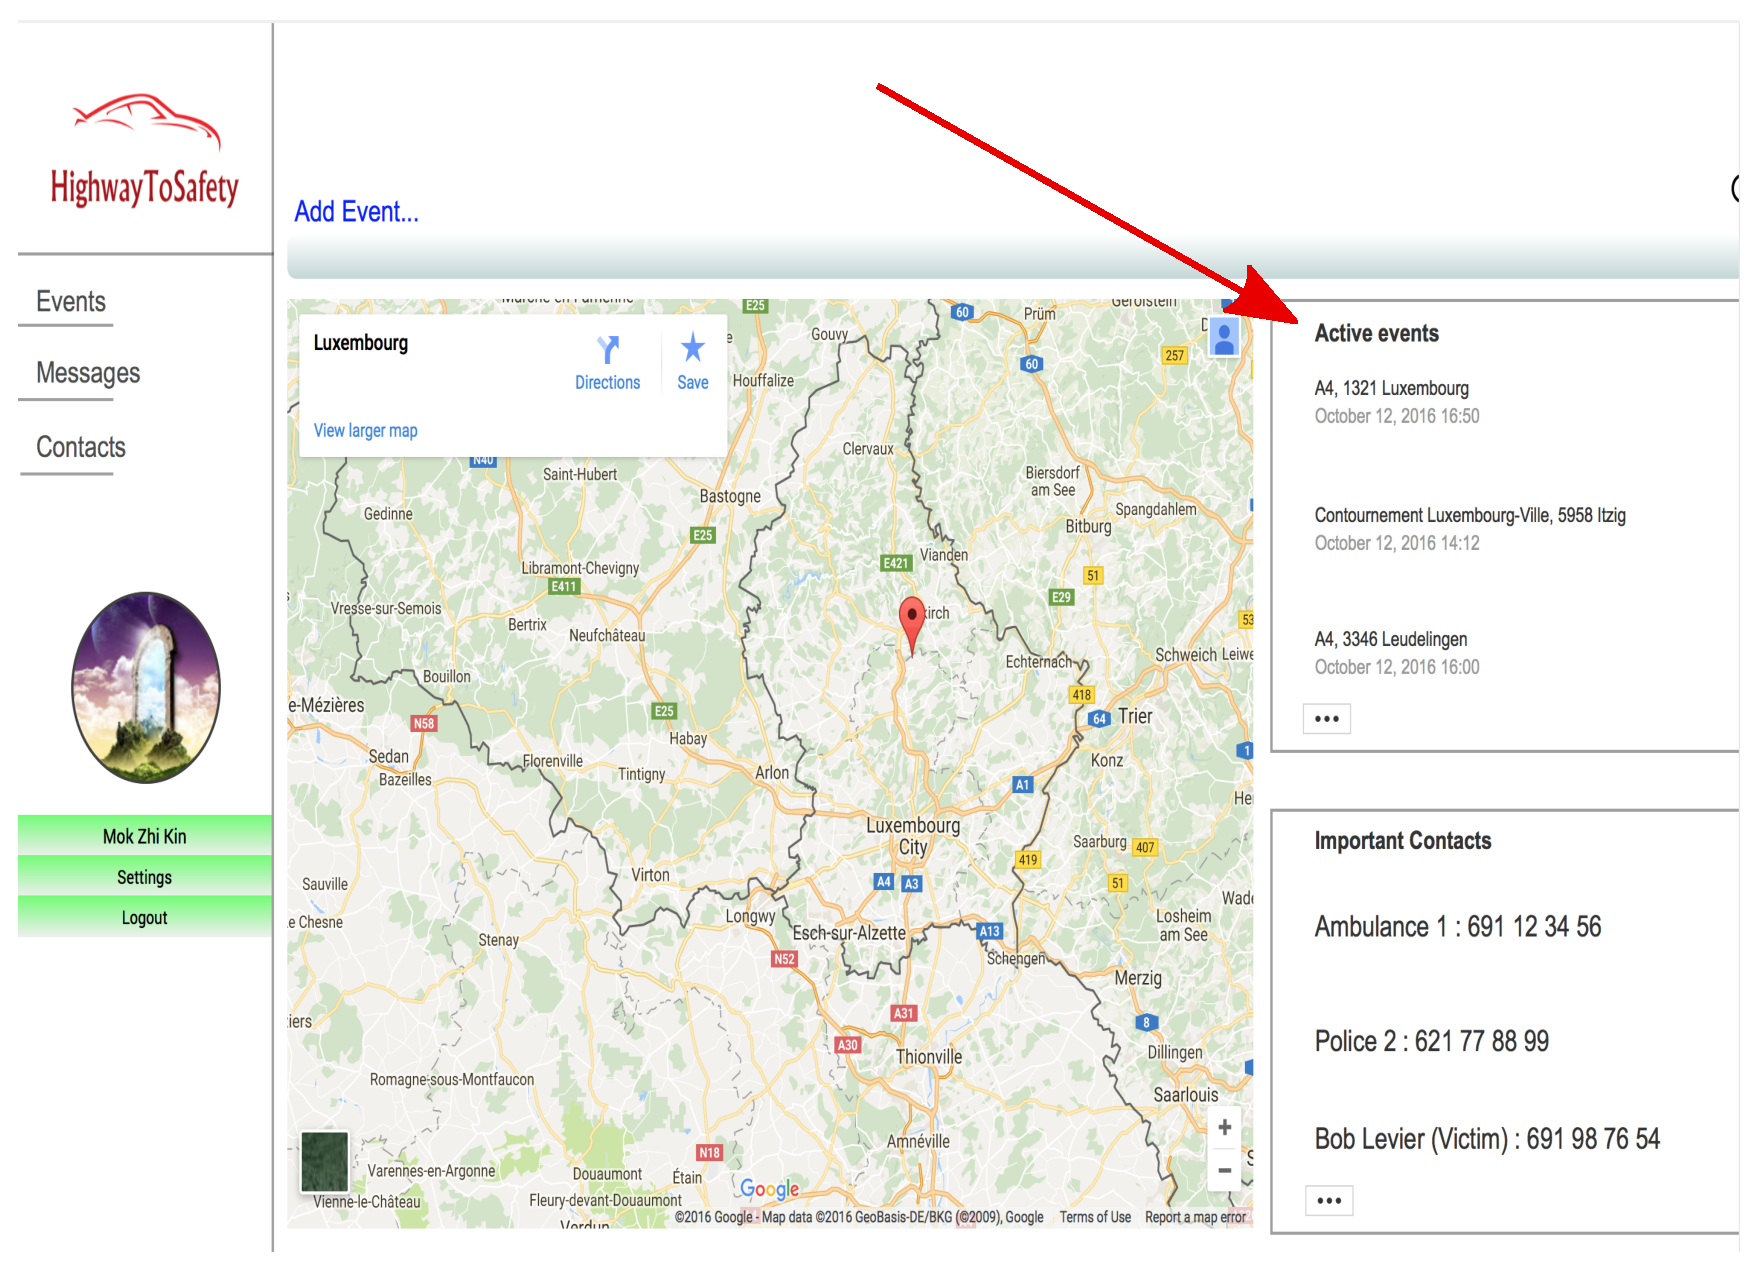
\includegraphics[width=0.9\textwidth]{Active_events.eps}
\end{figure}
\end{minipage}